\section{Facit}

\setcounter{opgave}{0}

\emph{NB: Alle elektriske ladninger er angivet i enheder af elementarladningen \si{\elementarycharge}, hvilket er underforstået hele vejen gennem facitlisten.}\\

\begin{opgave}{Neutrinoernes vilde verden}
    \begin{itemize}
        \item $\nu_\mathrm{e}$: Elektronneutrino
        \item $\nu_\mu$: Myonneutrino
        \item $\nu_\tau$: Tauneutrino
        \item $\bar{\nu}_\mathrm{e}$: Antielektronneutrino
        \item $\bar{\nu}_\mu$: Antimyonneutrino
        \item $\bar{\nu}_\tau$: Antitauneutrino
    \end{itemize}
    %%
    \opg Neutrinoer har ingen farveladning eller elektrisk ladning, og de kan derfor ikke måles med den stærke eller den elektromagnetisk vekselvirkning. De kan derfor kun måles med den svage vekselvirkning, men disse partikelreaktioner er ikke ret sandsynlige. Derfor er man nød til at have meget store detektorer for overhovedet at kunne måle neutrinoerne, og derudover skal man også kunne sikre sig, at det ikke er alt mulig andet end neutrinoer man observerer.
    \opg Leptontalsbevarelse og teknisk set også impulsbevarelse. Det sidste skal forstås ved at reaktionen hypotetisk set godt kunne bevare impuls uden neutrinoen, men at tilstedeværelsen af neutrinoen påvirker bevægelsesretningen af de andre reaktionsprodukter, så neutrinoen er nødvendig for at impulsbevarelse er opfyldt i eksperimenter.
\end{opgave}

\begin{opgave}{Leptonfamilier}
    \opg $\mu^-$, $\mu^+$, $\nu_\mu$ og $\bar{\nu}_\mu$.
    \opg Deres masse er større, og de er derfor mere energirige.
    \opg Elektronfamilien er mest stabil, da deres masser og dermed deres energi er mindst.
\end{opgave}

\begin{opgave}{Kvarksammensætninger}
    De to kvarker i første generation er u og d, og de har hver deres antipartikel, henholdsvis $\bar{\mathrm u}$ og $\bar{\mathrm d}$. Den elektriske ladningen af u-kvarken og dens antipartikel er henholdsvis $\pm2/3$, mens det for nedkvarken er $\mp1/3$. Da
    \begin{align*}
        2\cdot\left(-\frac{1}{3}\right) + \frac{2}{3} = -\left[2\cdot\left(-\frac{1}{3}\right) + \frac{2}{3}\right] = 0,
    \end{align*}
    skal man bruge enten to partikler med elektrisk ladningen $-1/3$ og en partikel med elektrisk ladning $2/3$, eller en partikel med elektrisk ladning $-2/3$ og 2 med elektrisk ladning $1/3$. Det kan man gøre på følgende måder:
    \begin{itemize}
        \item udd
        \item $\bar{\mathrm u}\bar{\mathrm d}\bar{\mathrm d}$
    \end{itemize}
\end{opgave}

\begin{opgave}{$\mathbf{\gamma}$-henfald af atomer}
    \opg Der udsendes en foton, som er den elektromagnetiske boson, hvorfor henfaldet er elektromagnetisk.
    \opg Bosonen i figur \ref{fig:betaminus} er W$^-$-bosonen, som tilhører den svage vekselvirkning.
    \opg Se figur \ref{fig:betaminus_med_kvarker}.
    \opg Den letteste måde at tegne Feynmandiagrammet på er at benytte, at man for alle knudepunkter må omdanne alle partikler til deres antipartikler. Det betyder, at det eneste man skal gøre er at bytte om på en op- og en nedkvark, samt at skifte bosonen og hvad den henfalder til, til deres antipartikler, se figur \ref{fig:betaplus}.
    \opg Forskellen er netop, at den boson der udsendes i de to reaktioner er hinandens antipartikler, hvorfor henfaldsprodukterne også blot er hinandens antipartikler.
\end{opgave}

\begin{figure} [h!]
    \centering
    \begin{subfigure}[t]{.4\textwidth}
        \begin{tikzpicture}
            \draw[fermion] (-2,0) node[anchor = east]{d} -- (0,0);
            \draw[fermion] (0,0) -- (3,0) node[anchor = west]{u};
            \draw[boson] (0,0) -- (1,1);
            \draw[fermion] (1,1) -- (3,1)node[anchor = west]{$e^-$};
            \draw[fermion] (3,1.6) node[anchor = west]{$\bar{\nu}_e$} -- (1,1);
            \draw (0.6,0.4) node[anchor=south east]{$\mathrm{W}^-$};
            \draw[fermion] (-2,-.5) node[anchor = east]{u} -- (3,-.5)node[anchor = west]{u};
            \draw[fermion] (-2,-1) node[anchor = east]{d} -- (3,-1)node[anchor = west]{d};
            \draw[line width = 0.5mm] (-2.25,-1.25) -- (-2.5,-1.25) -- (-2.5,0.25) -- (-2.25,0.25);
            \draw (-2.5,-0.5) node[anchor = east]{n};
            \draw[line width = 0.5mm] (3.25,-1.25) -- (3.5,-1.25) -- (3.5,0.25) -- (3.25,0.25);
            \draw (3.5,-0.5) node[anchor = west]{p};
            \vertex{0,0};
            \vertex{1,1};
        \end{tikzpicture}
    \caption{Feynmandiagram for  $\beta^-$-henfaldet med kvarker.}
    \label{fig:betaminus_med_kvarker}
    \end{subfigure}
    %
    \hfill
    %
    \begin{subfigure}[t]{0.4\textwidth}
        \centering
            \begin{tikzpicture}
                \draw[fermion] (-2,0) node[anchor = east]{u} -- (0,0);
                \draw[fermion] (0,0) -- (3,0) node[anchor = west]{d};
                \draw[boson] (0,0) -- (1,1);
                \draw[fermion] (3,1)node[anchor = west]{$e^+$} -- (1,1);
                \draw[fermion] (1,1) -- (3,1.6)node[anchor = west]{$\nu_e$};
                \draw (0.6,0.4) node[anchor=south east]{$\mathrm{W}^+$};
                \draw[fermion] (-2,-.5) node[anchor = east]{u} -- (3,-.5)node[anchor = west]{u};
                \draw[fermion] (-2,-1) node[anchor = east]{d} -- (3,-1)node[anchor = west]{d};
                \draw[line width = 0.5mm] (-2.25,-1.25) -- (-2.5,-1.25) -- (-2.5,0.25) -- (-2.25,0.25);
                \draw (-2.5,-0.5) node[anchor = east]{p};
                \draw[line width = 0.5mm] (3.25,-1.25) -- (3.5,-1.25) -- (3.5,0.25) -- (3.25,0.25);
                \draw (3.5,-0.5) node[anchor = west]{n};
                \vertex{0,0};
                \vertex{1,1};
            \end{tikzpicture}
        \caption{Feynmandiagram for  $\beta^+$-henfaldet med kvarker.}
        \label{fig:betaplus}
    \end{subfigure}
    \caption{Feynmandiagram for begge $\beta$-henfald}
    \label{fig:feynman_beta}
\end{figure}

\begin{opgave}{Bevarelseslove}
    \opg Kig på følgende reaktioner og bestem, om de kan lade sig gøre eller ej.
    \begin{enumerate}
        \item Nej, pga. ladningsbevarelse og leptontalsbevarelse.
        \item Nej, pga. lepton- og baryontalsbevarelse.
        \item Nej, pga. ladningsbevarelse.
        \item Nej, pga. ladningsbevarelse.
        \item Ja, da alle bevarelseslove er opfyldt.
        \item Ja, da alle bevarelseslove er opfyldt.
        \item Nej, pga. baryontalsbevarelse.
    \end{enumerate}
\end{opgave}

\begin{opgave}{Dannelse af myoner}
    \opg For at opfylde ladningsbevarelse skal den være positivt ladet. For at opfylde leptontalsbevarelse skal det være en lepton. Den eneste positivt ladet lepton i myonfamilien er $\mu^+$, hvorfor det må være den anden elementarpartikel.
    \opg Se figur \ref{fig:myonpardannelse}.
\end{opgave}

\begin{figure} [h!]
        \centering
        \begin{tikzpicture}
            \draw[fermion] (1.5,-1) node[anchor = north west]{$\mu^+$} -- (0,0);
            \draw[fermion] (0,0) -- (1.5,1) node [anchor = south west]{$\mu^-$};
            \draw[photon] (0,0) -- (-1.5,0)node[anchor = east]{$\gamma$};
            \vertex{0,0};
        \end{tikzpicture}
        \caption{Feynmandiagram for dannelsen af et myon- antimyonpar.}
        \label{fig:myonpardannelse}
    \end{figure}

\begin{opgave}{Rotation af knudepunkter i Feynmandiagrammer} \label{opg:rotation_af_Feynman}
    \opg Der produceres en antielektronneutrino, se figur \ref{fig:Wvertex_rot}
    \opg Positiv, da den ikke har skiftet side af knudepunktet.
    \opg For at bevare leptontallet bliver det en elektronneutrino, $\nu_\mathrm{e}.$
    \opg For at bevare ladningen, skal denne være negativ.
    \opg Begge leptoner krydser knudepunktet, hvorfor de bliver til deres antipartikel. De er dog hinandens antipartikel, hvorfor de bliver til hinanden. Fotonen er sin egen antipartikel, hvorfor den bliver til sig selv. At det ser ud som om der ikke ændres ladninger, skyldes blot at begge ladninger ændres og bliver til hinanden.
\end{opgave}

\begin{figure}[h!]
        \centering
        \begin{tikzpicture}
            \draw[fermion] (0,0) -- (-1.5,0)node[anchor = east]{$\mathrm{e}^+$};
            \draw[boson] (0,0) -- (1.5,1)node[anchor = west]{$\mathrm{W}^+$};
            \draw[fermion] (1.5,-1)node[anchor = west]{$\bar{\nu}_\mathrm{e}$} -- (0,0);
            \vertex{0,0};
        \end{tikzpicture}
        \caption{Udsendelse af en $\mathrm{W}^+$-boson.}
        \label{fig:Wvertex_rot}
    \end{figure}

\begin{opgave}{Kvarkkobling} \label{opg:Kvarkkobling}
    \opg Den svage vekselvirkning kobler så at sige lodret og diagonalt, se figur \ref{fig:opg35}.
    \opg Se figur \ref{fig:topkvark}.
    \opg Positiv, $+1$, for at opfylde ladningsbevarelse.
    \opg Se figur \ref{fig:s_anti_c_annihilation}.
    \opg Negativ, $-1$, for at opfylde ladningsbevarelse.
    \opg W-- og Z--bosoner er ikke stabile, og de henfalder typisk til det lettest mulige produkt. I tilfældet af W$^-$ er det en elektron og en antielektronneutrino.
\end{opgave}

\begin{figure} [h!]
  \centering
  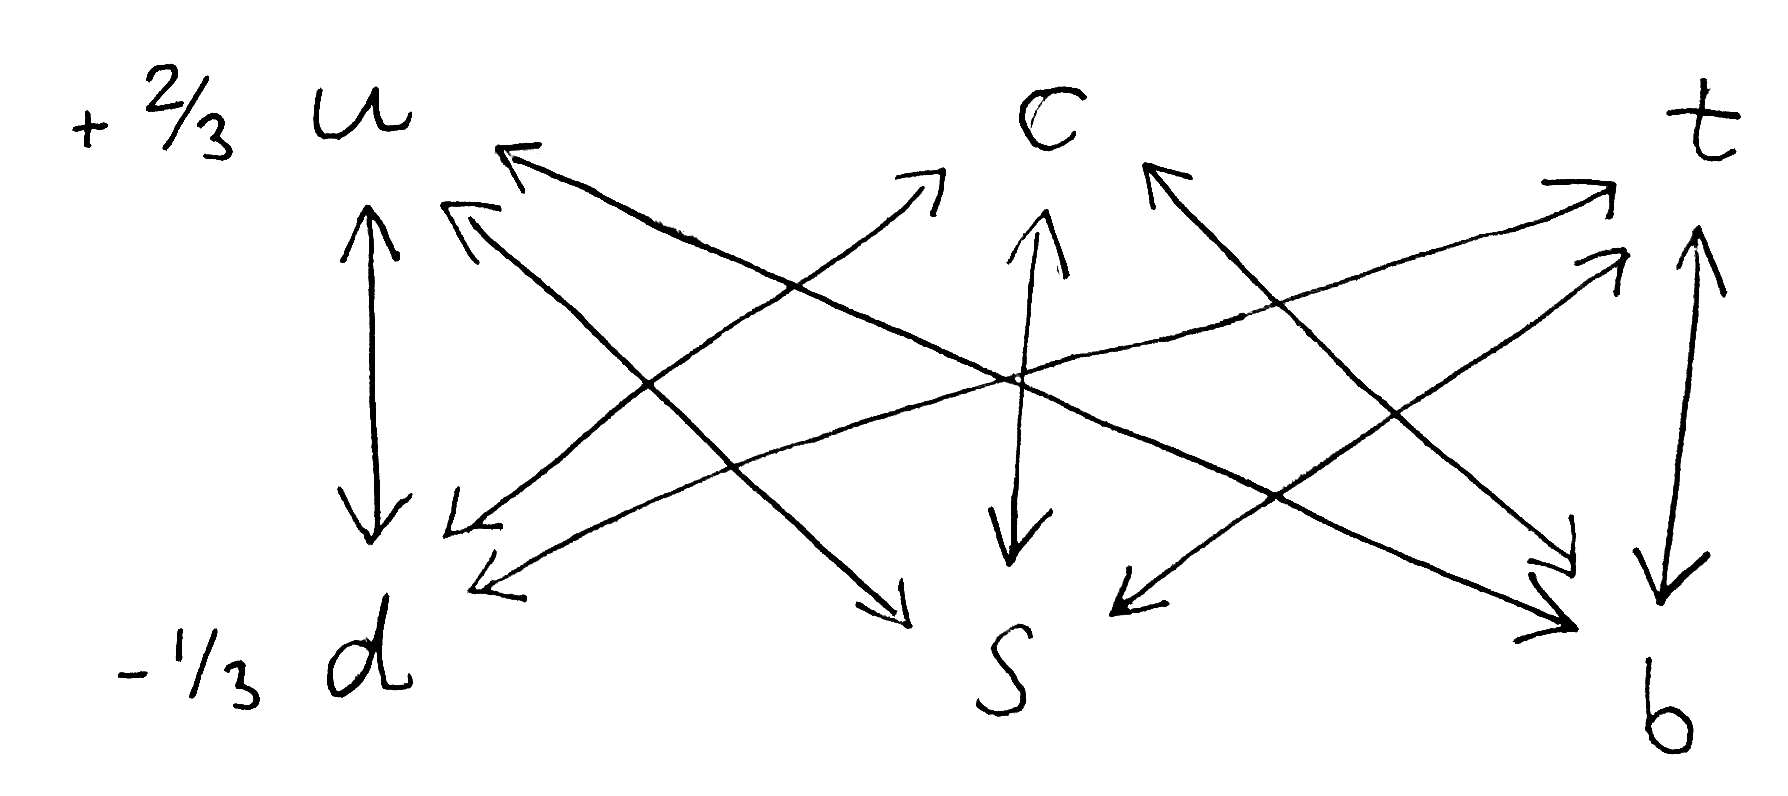
\includegraphics[width=0.4\textwidth]{facit/figurer/kvarkkobling.png}
  \caption{Kvarkomdannelser som $W$ kan lave.}
  \label{fig:opg35}
\end{figure}

\begin{figure} [h!]
    \centering
	\begin{subfigure}[t]{0.47\textwidth}
	    \centering
	    \begin{tikzpicture}
            \draw[fermion] (-2,0) node[anchor = east]{t} -- (0,0);
            \draw[fermion] (0,0) -- (3,0) node[anchor = west]{b};
            \draw[boson] (0,0) -- (1,1);
            \draw[fermion] (3,1)node[anchor = west]{$e^+$} -- (1,1);
            \draw[fermion] (1,1) -- (3,1.6)node[anchor = west]{$\nu_e$};
            \draw (0.6,0.4) node[anchor=south east]{$\mathrm{W}^+$};
            \vertex{0,0};
            \vertex{1,1};
        \end{tikzpicture}
    \caption{Henfald af topkvarken}
    \label{fig:topkvark}
    \end{subfigure}
    %
    \hfill
    %
    \begin{subfigure}[t]{0.47\textwidth}
        \centering
        \begin{tikzpicture}
		    \draw[fermion] (0,0) -- (-1.5,1)node[anchor = east]{$\bar{\mathrm{c}}$};
            \draw[boson] (0,0) -- (1.5,0);
            \draw[fermion] (-1.5,-1)node[anchor = east]{s} -- (0,0);
            \draw (.75,0)node[anchor = south]{$\mathrm{W}^-$};
		    \draw[fermion] (1.5,0) -- (3,1)node[anchor = west]{e$^-$};
            \draw[fermion] (3,-1)node[anchor = west]{$\bar{\nu}_\mathrm{e}$} -- (1.5,0);
            \vertex{1.5,0};
            \vertex{0,0};
	    \end{tikzpicture}
        \caption{Annihilation af en strange- og anticharmkvark.}
        \label{fig:s_anti_c_annihilation}
        \end{subfigure}
        \caption{Figur til opgave om kvarkkobling.}
\end{figure}
    
\begin{opgave}{Feynman-diagrammer: En sand kunstart}
    \opg Ladningen af $W$ er -1.
    \opg Den ene kvark udsender en gluon og passerer derefter uændret. Gluonen henfalder til et kvark/anti-kvark-par. Den anden kvark i $D^-$-mesonen ændres under udsendelse af en $W^-$. Denne $W^-$ henfalder og skaber to nye kvarker.
    \opg For at finde kvarksammensætningen af en sammenssat partikels antipartikel, ændrer man blot alle partikler til antipartikler:
    \begin{align*}
        &\mathrm K^+(\mathrm u \bar{\mathrm{s}}) \rightarrow K^-(\bar{\mathrm{u}} \mathrm s) \\
        &\pi^+(\mathrm u \bar{\mathrm{d}}) \rightarrow \pi^-(\bar{\mathrm{u}} \mathrm d)
    \end{align*}
    Herfra er det at lege lidt med Feynmandiagrammet fra tidligere, figur \ref{fig:quark_inter}, for at få figur \ref{fig:d-k-}.
    \opg K$^+$ og $\pi^-$, da den delen af reaktionen der indeholder en W--boson er mest sandsynlig, når henfaldet af $\bar{\text{c}}$ sker til en kvark af samme generation. Det er altså mest sandsynligt, at $\bar{\mathrm c} \rightarrow \bar{\mathrm s}$ og W$^- \rightarrow \bar{\mathrm u}$d, end at $\bar{\mathrm c} \rightarrow \bar{\mathrm d}$ og W$^- \rightarrow \bar{\mathrm u}$s.
\end{opgave}

\begin{figure} [h!]
        \centering
        \begin{tikzpicture}
            \draw[fermion] (0,0.25) node[anchor = east]{d}-- (2,1.5);
            \draw[fermion] (2,-1) -- (0,-0.25)node[anchor = east]{$\bar{\mathrm{c}}$};
            \draw[fermion] (6,-0.25) node[anchor=west]{$\bar{\mathrm d}$} -- (2,-1);
            \draw[fermion] (2,1.5) -- (6,2.25) node[anchor = west]{d};
            \draw[gluon] (2,1.5) -- (4,0.75);
            \draw (3,1) node[anchor = north east]{g};
            \draw[fermion] (6,1.75) node[anchor = west]{$\bar{\mathrm u}$} -- (4,0.75);
            \draw[fermion] (4,0.75) -- (6,0.25) node[anchor = west]{u};
            \draw[boson] (2,-1) -- (4,-2);
            \draw[fermion] (4,-2) -- (6,-1.75) node[anchor = west]{s};
            \draw[fermion] (6,-2.25) node[anchor = west]{$\bar{\mathrm u}$} -- (4,-2);
            \draw (3.2,-1.6) node[anchor = north east]{$\mathrm{W}^-$};
            \vertex{2,1.5};
            \vertex{2,-1};
            \vertex{4,0.75};
            \vertex{4,-2};
            \draw[line width = 0.5mm] (-0.25,-0.5) -- (-0.5,-0.5) -- (-0.5,0.5) -- (-0.25,0.5);
            \draw (-0.5,0) node[anchor = east]{$\mathrm{D}^-$};
            \draw[line width = 0.5mm] (6.25,-0.6) -- (6.5,-0.6) -- (6.5,0.5) -- (6.25,0.5);
            \draw[line width = 0.5mm] (6.25,1.5) -- (6.5,1.5) -- (6.5,2.5) -- (6.25,2.5);
            \draw[line width = 0.5mm] (6.25,-1.5) -- (6.5,-1.5) -- (6.5,-2.5) -- (6.25,-2.5);
            \draw (6.5,0) node[anchor = west]{$\pi^+$};
            \draw (6.5,2) node[anchor = west]{$\pi^-$};
            \draw (6.5,-2) node[anchor = west]{K$^-$};
        \end{tikzpicture}
        \caption{Henfaldet af D$^-$-mesonen til K$^+$, $\pi^-$ og $\pi^+$.}
        \label{fig:d-k-}
\end{figure}

\begin{opgave}{Flere Feynmandiagrammer}
    \opg Se figur \ref{fig:b-}.
    \opg Se figur \ref{fig:sigma-}.
    \opg Se figur \ref{fig:delta0}.
    \opg Se figur \ref{fig:ds+}.
    \opg Se figur \ref{fig:omega-}.
\end{opgave}

\begin{figure} [h!]
    \centering
    \begin{subfigure}[t]{.4\textwidth}
    	\begin{tikzpicture}
    		\draw[fermion] (4.5,1.5) node[anchor = west]{$\bar{\mathrm u}$} -- (0,.5) node[anchor = east]{$\bar{\mathrm u}$};
		    \draw[fermion] (0,0) node[anchor = east]{b}-- (1.5,0);
            \draw[fermion] (1.5,0) -- (4.5,1) node[anchor = west]{c};
            \draw[boson] (1.5,0) -- (3,-0.75);
            \draw (2.5,-.5) node[anchor = north east]{W$^-$};
            \draw[fermion] (4.5,-0.5) node[anchor = west]{$\bar{\mathrm u}$} -- (3,-0.75);
            \draw[fermion] (3,-0.75) -- (4.5,-1.05) node[anchor = west]{d};
		    \vertex{1.5,0};
		    \vertex{3,-0.75};
            \draw[line width = 0.5mm] (-.25,0.8) -- (-.5,0.8) -- (-.5,-.25) -- (-.25,-.25);
            \draw (-1.2,0.25) node[anchor = west]{B$^-$};
            \draw[line width = 0.5mm] (4.75,1.8) -- (5,1.8) -- (5,.8) -- (4.75,.8);
            \draw (5,1.3) node[anchor = west]{D$^0$};
            \draw[line width = 0.5mm] (4.75,-0.2) -- (5,-0.2) -- (5,-1.3) -- (4.75,-1.3);
            \draw (5,-.7) node[anchor = west]{$\rho^-$};
		\end{tikzpicture}
	    \caption{$\text{B}^- (\mathrm b\bar{\mathrm u}) \longrightarrow \text{D}^0(\mathrm c\bar{\mathrm u}) + \rho^-(\mathrm d\bar{\mathrm u})$}
    	\label{fig:b-}
    \end{subfigure}
    %
    \hfill
    %
    \begin{subfigure}[t]{.4\textwidth}
    	\begin{tikzpicture}
            \draw[fermion] (-1.5,0) node[anchor = east]{d} -- (0,0);
            \draw[fermion] (0,0) -- (3,0) node[anchor = west]{u};
            \draw[boson] (0,0) -- (1,1);
            \draw[fermion] (1,1) -- (3,1)node[anchor = west]{e$^-$};
            \draw[fermion] (3,1.6) node[anchor = west]{$\bar{\nu}_e$} -- (1,1);
            \draw (0.6,0.4) node[anchor=south east]{$\mathrm{W}^-$};
            \draw[fermion] (-1.5,-.5) node[anchor = east]{s} -- (3,-.5)node[anchor = west]{s};
            \draw[fermion] (-1.5,-1) node[anchor = east]{d} -- (3,-1)node[anchor = west]{d};
            \draw[line width = 0.5mm] (-1.75,-1.25) -- (-2,-1.25) -- (-2,0.25) -- (-1.75,0.25);
            \draw (-2,-0.5) node[anchor = east]{$\Sigma^-$};
            \draw[line width = 0.5mm] (3.25,-1.25) -- (3.5,-1.25) -- (3.5,0.25) -- (3.25,0.25);
            \draw (3.5,-0.5) node[anchor = west]{$\Lambda^0$};
            \vertex{0,0};
            \vertex{1,1};
        \end{tikzpicture}
	    \caption{$\Sigma^-(\mathrm{dds}) \longrightarrow \Lambda^0 (\mathrm{uds}) + \mathrm{e}^- + \bar{\nu}_\mathrm{e}$}
    	\label{fig:sigma-}
    \end{subfigure}
    %
    \hfill
    %
    \begin{subfigure}[t]{.4\textwidth}
    	\begin{tikzpicture}
            \draw[fermion] (-2,0) node[anchor = east]{d} -- (0,0);
            \draw[fermion] (0,0) -- (3,0) node[anchor = west]{u};
            \draw[boson] (0,0) -- (1,1);
            \draw[fermion] (1,1) -- (3,1)node[anchor = west]{\aq{u}};
            \draw[fermion] (3,1.6) node[anchor = west]{u} -- (1,1);
            \draw (0.6,0.4) node[anchor=south east]{$\mathrm{W}^-$};
            \draw[fermion] (-2,-.5) node[anchor = east]{u} -- (3,-.5)node[anchor = west]{u};
            \draw[fermion] (-2,-1) node[anchor = east]{d} -- (3,-1)node[anchor = west]{d};
            \draw[line width = 0.5mm] (3.25,.7) -- (3.5,.7) -- (3.5,1.85) -- (3.25,1.85);
            \draw (3.5,1.3) node[anchor = west]{$\pi^-$};
            \draw[line width = 0.5mm] (-2.25,-1.5) -- (-2.5,-1.5) -- (-2.5,0.25) -- (-2.25,0.25);
            \draw (-2.5,-0.5) node[anchor = east]{$\Delta^0$};
            \draw[line width = 0.5mm] (3.25,-1.25) -- (3.5,-1.25) -- (3.5,0.25) -- (3.25,0.25);
            \draw (3.5,-0.5) node[anchor = west]{p};
            \vertex{0,0};
            \vertex{1,1};
        \end{tikzpicture}
	    \caption{$\Delta^0 (\mathrm{udd}) \longrightarrow \mathrm{p} + \pi^- (\mathrm d\bar{\mathrm u})$}
    	\label{fig:delta0}
    \end{subfigure}
    %
    \hfill
    %
    \begin{subfigure}[t]{.4\textwidth}
    	\begin{tikzpicture}
    		\draw[fermion] (4.5,1.5) node[anchor = west]{$\bar{\mathrm s}$} -- (0,.5) node[anchor = east]{$\bar{\mathrm s}$};
		    \draw[fermion] (0,0) node[anchor = east]{c}-- (1.5,0);
            \draw[fermion] (1.5,0) -- (4.5,1) node[anchor = west]{s};
            \draw[boson] (1.5,0) -- (3,-0.75);
            \draw (2.5,-0.5) node[anchor = north east]{W$^+$};
            \draw[fermion] (4.5,-0.5) node[anchor = west]{$\bar{\mathrm d}$} -- (3,-0.75);
            \draw[fermion] (3,-0.75) -- (4.5,-1.05) node[anchor = west]{u};
		    \vertex{1.5,0};
		    \vertex{3,-0.75};
            \draw[line width = 0.5mm] (-.25,0.8) -- (-.5,0.8) -- (-.5,-.25) -- (-.25,-.25);
            \draw (-1.2,0.25) node[anchor = west]{D$_\mathrm{s}^+$};
            \draw[line width = 0.5mm] (4.75,1.8) -- (5,1.8) -- (5,.8) -- (4.75,.8);
            \draw (5,1.3) node[anchor = west]{$\varphi$};
            \draw[line width = 0.5mm] (4.75,-0.2) -- (5,-0.2) -- (5,-1.3) -- (4.75,-1.3);
            \draw (5,-.7) node[anchor = west]{$\rho^+$};
		\end{tikzpicture}
	    \caption{$\mathrm D_\mathrm{s}^+ (\mathrm c\bar{\mathrm s}) \longrightarrow \varphi (\mathrm s\bar{\mathrm s}) + \rho^+ (\mathrm u\bar{\mathrm d})$}
    \label{fig:ds+}
    \end{subfigure}
    %
    \hfill
    %
    \begin{subfigure}[t]{.4\textwidth}
    	\begin{tikzpicture}
            \draw[fermion] (-2,0) node[anchor = east]{s} -- (-.5,.5);
            \draw[fermion] (1,0) -- (3,0) node[anchor = west]{d};
            \draw[boson] (-.5,.5) -- (1,0);
            \draw[fermion] (-.5,.5) -- (3,1.6)node[anchor = west]{u};
            \draw[fermion] (3,1.1)node[anchor = west]{\aq{u}} -- (1,0);
            \draw (0.35,-0.25) node[anchor=south east]{$\mathrm{W}^-$};
            \draw[fermion] (-2,-.5) node[anchor = east]{s} -- (3,-.5)node[anchor = west]{s};
            \draw[fermion] (-2,-1) node[anchor = east]{s} -- (3,-1)node[anchor = west]{s};
            \draw[line width = 0.5mm] (-2.25,-1.25) -- (-2.5,-1.25) -- (-2.5,0.3) -- (-2.25,0.3);
            \draw (-2.5,-0.5) node[anchor = east]{$\Omega^-$};
            \draw[line width = 0.5mm] (3.25,.8) -- (3.5,.8) -- (3.5,1.85) -- (3.25,1.85);
            \draw (3.5,1.3) node[anchor = west]{$\pi^0$};
            \draw[line width = 0.5mm] (3.25,-1.25) -- (3.5,-1.25) -- (3.5,0.3) -- (3.25,0.3);
            \draw (3.5,-0.5) node[anchor = west]{$\Xi^-$};
            \vertex{-0.5,.5};
            \vertex{1,0};
        \end{tikzpicture}
	    \caption{$\Omega^-(\mathrm{sss}) \longrightarrow \Xi^-(\mathrm{dss}) + \pi^0(\mathrm u\bar{\mathrm u})$}
    \label{fig:omega-}
    \end{subfigure}
    \caption{Forslag til løsninger til opgaven om flere Feynmandigrammer.}
    \label{fig:flere_feynman}
\end{figure}

\begin{figure}
    \centering
    \begin{subfigure}[t]{.4\textwidth}
        \begin{tikzpicture}
            \draw[fermion](0,0.2) node[anchor = east]{u} -- (1.5,1);
            \vertex{1.5,1};
            \draw[fermion] (1.5,1) -- (4.5,2.2)node[anchor = west]{u};
            \draw[gluon] (1.5,1)-- (3,0.5);
            \vertex{3,0.5};
            \draw (2.25,0.65)node[anchor= north]{g};
            \draw[fermion] (4.5,1.8) node[anchor = west]{$\bar{\mathrm{d}}$} -- (3,0.5);
            \draw[fermion] (3,0.5) -- (4.5,0.2)node[anchor = west]{d};
            \draw[fermion] (4.5,-0.2) node[anchor = west]{$\bar{\mathrm{u}}$} -- (1.5,-0.5);
            \vertex{1.5,-0.5};
            \draw[fermion] (1.5,-0.5) -- (0,-0.2) node[anchor = east]{$\bar{\mathrm{u}}$};
            \draw[boson] (1.5,-0.5) -- (3,-1.5);
            \vertex{3,-1.5};
            \draw[fermion] (3,-1.5) -- (4.5,-1) node[anchor = west]{e$^-$};
            \draw[fermion] (4.5,-2)node[anchor = west]{e$^+$} -- (3,-1.5);
            \draw (2,-.9)node[anchor = north]{Z$^0$};
            \draw (0,-0.3) -- (-0.1,-0.3);
            \draw[line width = 0.5mm] (-.25,0.5) -- (-.5,0.5) -- (-.5,-.5) -- (-.25,-.5);
            \draw (-1.2,0) node[anchor = west]{$\eta$};
            \draw[line width = 0.5mm] (4.75,0.5) -- (5.0,0.5) -- (5.0,-0.5) -- (4.75,-0.5);
            \draw (5.0,0)node[anchor = west]{$\pi^-$};
            \draw[line width = 0.5mm] (4.75,2.5) -- (5.0,2.5) -- (5.0,1.5) -- (4.75,1.5);
            \draw (5.0,2)node[anchor = west]{$\pi^+$};
        \end{tikzpicture}
        \caption{$\mathrm{\eta(u\bar u)\rightarrow\pi^+(u\bar{d}+\pi^-(d\bar u)+e^-+e^+}$}
    \end{subfigure}
    %
    \hfill
    %
	\begin{subfigure}[t]{0.47\textwidth}
        \centering
        \begin{tikzpicture}
            \draw[fermion] (-1.7,0) node[anchor = east]{$\tau^-$} -- (-.5,0);
            \draw[fermion] (-.5,0) -- (4,-1.5) node[anchor = west]{$\nu_\tau$};
            \draw[boson] (-.5,0) -- (0.25,1);
            \draw[gluon]  (1.3,-.2) -- (2.5,.5);
            \draw (1.7,.5) node[anchor south east]{g};
            \draw[fermion] (2.5,.5) -- (4,1.1)node[anchor = west]{d};
            \draw[fermion] (2.5,.5) -- (4,0)node[anchor = west]{$\bar{\mathrm d}$};
            \draw[fermion] (1.3,-.2) -- (4,-.5)node[anchor = west]{d};
            \draw[fermion] (.25,1) -- (1.3,-.2);
            \draw[fermion] (0.25,1) -- (4,1.6)node[anchor = west]{$\bar{\mathrm u}$};
            \draw (-.1,0.5) node[anchor=south east]{$\mathrm{W}^+$};
            \vertex{-.5,0};
            \vertex{0.25,1};
            \vertex{1.3,-.2};
            \vertex{2.5,.5};
            \draw[line width = 0.5mm] (4.25,1.9) -- (4.5,1.9) -- (4.5,.8) -- (4.25,.8);
            \draw (4.5,1.4)node[anchor = west]{$\pi^+$};
            \draw[line width = 0.5mm] (4.25,.3) -- (4.5,.3) -- (4.5,-.8) -- (4.25,-.8);
            \draw (4.5,-.2)node[anchor = west]{$\pi^0$};
        \end{tikzpicture}
    \caption{$\tau^- \longrightarrow \pi^+(\mathrm d\bar{\mathrm u}) + \pi^0(\mathrm d\bar{\mathrm d}) + \nu_\tau$}
    \label{fig:topkvark_2}
    \end{subfigure}
    %
    \hfill
    %
    \begin{subfigure}[t]{.47\textwidth}
	    \begin{tikzpicture}
		    \draw[fermion] (4.5,1.5) node[anchor = west]{$\bar{\mathrm s}$} -- (0,.5) node[anchor = east]{$\bar{\mathrm s}$};
	        \draw[fermion] (0,0) node[anchor = east]{b}-- (1.5,0);
            \draw[fermion] (1.5,0) -- (4.5,1) node[anchor = west]{u};
            \draw[gluon] (1.5,0) -- (3,-0.75);
            \draw (2.5,-.5) node[anchor = north east]{g};
            \draw[fermion] (4.5,-0.5) node[anchor = west]{$\bar{\mathrm u}$} -- (3,-0.75);
            \draw[fermion] (3,-0.75) -- (4.5,-1.05) node[anchor = west]{d};
	        \vertex{1.5,0};
	        \vertex{3,-0.75};
            \draw[line width = 0.5mm] (-.25,0.8) -- (-.5,0.8) -- (-.5,-.25) -- (-.25,-.25);
            \draw (-1.4,0.25) node[anchor = west]{K$^{*0}$};
            \draw[line width = 0.5mm] (4.75,1.8) -- (5,1.8) -- (5,.8) -- (4.75,.8);
            \draw (5,1.3) node[anchor = west]{K$^+$};
            \draw[line width = 0.5mm] (4.75,-0.2) -- (5,-0.2) -- (5,-1.3) -- (4.75,-1.3);
            \draw (5,-.7) node[anchor = west]{$\pi^-$};
	    \end{tikzpicture}
        \caption{$\text{K}^{*0} (\mathrm d\bar{\mathrm s}) \longrightarrow \text{K}^+(\mathrm u\bar{\mathrm s}) + \pi^-(\mathrm d\bar{\mathrm u})$}
	    \label{fig:k*0}
    \end{subfigure}
    %
    \hfill
    %
    \begin{subfigure}[t]{.47\textwidth}
        \begin{tikzpicture}
            \draw[line width = 0.5mm] (-.25,0.5) -- (-.5,0.5) -- (-.5,-.5) -- (-.25,-.5);
            \draw (-1.2,0) node[anchor = west]{K$^+$};
            \draw[fermion] (0,0.2)node[anchor=east]{u} arc(120:60:4.5) node[anchor = west]{u};
            \draw[line width = 0.5mm] (4.75,0.5) -- (5.0,0.5) -- (5.0,-0.5) -- (4.75,-0.5);
            \draw (5.0,0) node[anchor = west]{$\pi^+$};
            \draw[fermion] (0,-.2) node[anchor = east]{$\bar{\mathrm{s}}$} -- (1.5,-.2);
            \vertex{1.5,-.2};
            \vertex{3,-.2};
            \draw[boson] (1.5,-.2) arc(240:300:1.5);
            \draw[fermion] (1.5,-.2) arc(120:60:1.5);
            \draw[fermion] (3,-.2) -- (4.5,-.2) node[anchor=west]{$\bar{\mathrm{d}}$};
            \draw (2.25,0.6) node[anchor = north]{$\bar{\mathrm{u}}$};
            \draw (2.25,-1) node[anchor = south]{W$^+$};
        \end{tikzpicture}
        \caption{$\mathrm{K^+(u\bar{s})\rightarrow \pi^+(u\bar d)}$}
    \end{subfigure}
    \caption{Feynmandiagrammer til opgave \thechapter,\ref{opg:flere_feynman}.}
    \label{fig:flere_feynman}
\end{figure}
%
\begin{opgave}{Endnu flere Feynmandiagrammer} \label{opg:flere_feynman}
    \opg Kvarksammensætningen for $\pi^-$ findes ved at tage kvarksammensætningen for $\pi^+$ og ændre dem alle til deres antipartikler. Altså må $\pi^-$ have kvarksammensætningen $\bar{\text{u}}$d.
    \opg Reaktion 1 foregår ved en svag vekselvirkning. Reaktion 2 foregår ved en svag vekselvirkning. Reaktion 3 foregår ved en stærk vekselvirkning. Reaktion 4 foregår ved en svag vekselvirkning.
    \opg Se figur \ref{fig:flere_feynman}.
    \opg Reaktion 1 har 2 knudepunkter forbundet med en svag vekselvirkning. Reaktion 2 har 3 knudepunkter, 2 forbundet med en svag vekselvirkning og 1 forbundet med en stærk vekselvirkning. Reaktion 4 har 2 knudepunkter forbundet med en svag vekselvirkning.
    \opg Da der ikke er nogle af reaktionerne, som indeholder mere end en enkelt svag vekselvirkning (altså kun en W$^\pm$ eller Z$^0$), så der er ikke nogle af dem, der er så usandsynlige, at de aldrig sker.
\end{opgave}\\

\begin{opgave}{Reaktionssandsynlighed}
    \opg Stærk pga. gluonen.
    \opg Se figur \ref{fig:u-henfald2}.
    \opg W$^\pm$ da den er ladet, hvilket ville bryde med ladningsbevarelse.
    \opg Af afsnit 6.4.2 %\ref{sec:reaktionssandsynlighed} 
    er sandsynlighedsrækkefølgen:
    \begin{enumerate}
        \item Stærk vekselvirkning, figur 6.12.%\ref{fig:u-henfald}.
        \item Elektromagnetisk vekselvirkning, figur \ref{fig:u-henfald-s}.
        \item Svag vekselvirkning, figur \ref{fig:u-henfald-w}.
    \end{enumerate}
    \opg Alle tre bosoner henfalder til et vilkårlig kvark- antikvarkpar, deriblandt d$\bar{\mathrm{d}}$.
\end{opgave}

\begin{figure} [h!]
    \centering
    \begin{subfigure}{.47\textwidth}
    	\begin{tikzpicture}
		    \draw[fermion] (0,0) node[anchor = east]{u}-- (2,0);
            \draw[fermion] (2,0) -- (6,1) node[anchor = west]{u};
            \draw[photon] (2,0) -- (4,-0.75);
            \draw (3,-0.5) node[anchor = north east]{$\gamma$};
            \draw[fermion] (6,-0.5) node[anchor = west]{$\bar{\mathrm u}$} -- (4,-0.75);
            \draw[fermion] (4,-0.75) -- (6,-1.05) node[anchor = west]{u};
		    \vertex{2,0};
		    \vertex{4,-0.75};
            \draw[line width = 0.5mm] (6.25,-0.2) -- (6.5,-0.2) -- (6.5,-1.3) -- (6.25,-1.3);
            \draw (6.5,-.7) node[anchor = west]{$\pi^0$};
		\end{tikzpicture}
	    \caption{Elektromagnetisk henfald af en højenergikvark.}
    	\label{fig:u-henfald-s}
    \end{subfigure}
    %
    \hfill
    %
    \begin{subfigure}{.47\textwidth}
    	\begin{tikzpicture}
		    \draw[fermion] (0,0) node[anchor = east]{u}-- (2,0);
            \draw[fermion] (2,0) -- (6,1) node[anchor = west]{u};
            \draw[gluon] (2,0) -- (4,-0.75);
            \draw (3,-0.5) node[anchor = north east]{Z$^0$};
            \draw[fermion] (6,-0.5) node[anchor = west]{$\bar{\mathrm u}$} -- (4,-0.75);
            \draw[fermion] (4,-0.75) -- (6,-1.05) node[anchor = west]{u};
		    \vertex{2,0};
		    \vertex{4,-0.75};
            \draw[line width = 0.5mm] (6.25,-0.2) -- (6.5,-0.2) -- (6.5,-1.3) -- (6.25,-1.3);
            \draw (6.5,-.7) node[anchor = west]{$\pi^0$};
		\end{tikzpicture}
	    \caption{Svagt henfald af en højenergikvark.}
    	\label{fig:u-henfald-w}
    \end{subfigure}
    \caption{Henfald af en højenergikvark.}
    \label{fig:u-henfald2}
\end{figure}